% Set the document class and theme
\documentclass[notheorems]{beamer}

\setbeamertemplate{theorem}[ams style]
\setbeamertemplate{theorems}[numbered]

\makeatletter
    \ifbeamer@countsect
      \newtheorem{theorem}{\translate{Theorem}}[section]
    \else
      \newtheorem{theorem}{\translate{Theorem}}
    \fi
    \newtheorem{corollary}{\translate{Corollary}}
    \newtheorem{fact}{\translate{Fact}}
    \newtheorem{lemma}{\translate{Lemma}}
    \newtheorem{problem}{\translate{Problem}}
    \newtheorem{solution}{\translate{Solution}}

    \theoremstyle{definition}
    \newtheorem{definition}{\translate{Definition}}
    \newtheorem{definitions}{\translate{Definitions}}

    \theoremstyle{example}
    \newtheorem{example}{\translate{Example}}
    \newtheorem{examples}{\translate{Examples}}

    % Compatibility
    \newenvironment{Lemma}{\begin{lemma}}{\end{lemma}}
    \newenvironment{Proof}{\begin{proof}}{\end{proof}}
    \newenvironment{Theorem}{\begin{theorem}}{\end{theorem}}
    \newenvironment{Problem}{\begin{problem}}{\end{problem}}
    \newenvironment{Corollary}{\begin{corollary}}{\end{corollary}}
    \newenvironment{Example}{\begin{example}}{\end{example}}
    \newenvironment{Examples}{\begin{examples}}{\end{examples}}
    \newenvironment{Definition}{\begin{definition}}{\end{definition}}
\makeatother

\usetheme{Madrid}
\useoutertheme{miniframes} % Alternatively: miniframes, infolines, split
\useinnertheme{circles}

\definecolor{IITHorange}{RGB}{243, 130, 33} % UBC Blue (primary)
\definecolor{IITHyellow}{RGB}{254, 203, 10} % UBC Grey (secondary)

\setbeamercolor{palette primary}{bg=IITHorange,fg=white}
\setbeamercolor{palette secondary}{bg=IITHorange,fg=white}
\setbeamercolor{palette tertiary}{bg=IITHorange,fg=white}
\setbeamercolor{palette quaternary}{bg=IITHorange,fg=white}
\setbeamercolor{structure}{fg=IITHorange} % itemize, enumerate, etc
\setbeamercolor{section in toc}{fg=IITHorange} % TOC sections

% Override palette coloring with secondary
\setbeamercolor{subsection in head/foot}{bg=IITHyellow,fg=white}

\setbeamertemplate{caption}[numbered]
\setbeamertemplate{theorems}[numbered]

\usepackage{./presentation_macros}

\title{The Retracing Boomerang Attack}
\date{April 28, 2025}
\author{Gautam Singh}
\institute[IITH]{Indian Institute of Technology Hyderabad}

\begin{document}
    
    \begin{frame}
        \titlepage
    \end{frame}
    
    \begin{frame}
        \tableofcontents
    \end{frame}
    
    \section{Introduction}
    \label{sec:intro}
    
    \begin{frame}[<+->]{Introduction}
        \begin{enumerate}
            \item Broke the record for 5-round AES when it was
            published.
            \item Brings the attack complexity down to \(2^{16.5}\)
            encryptions.
            \item Uncovers a hidden relationship between boomerang attacks and
            two other cryptanalysis techniques: yoyo game and mixture
            differentials.
        \end{enumerate}
    \end{frame}

    \section{Preliminaries}
    \label{sec:prelims}

    \subsection{Boomerang Attacks}
    \label{subsec:boomerang}

    \begin{frame}{The Boomerang Attack}
        \begin{columns}
            \begin{column}{0.7\textwidth}
                \begin{enumerate}
                    \item<1-> Typically split the encryption function as \(E =
                    E_1 \circ E_0\), with differential trails for each
                    sub-cipher.
                    \item<2-> We can build a distinguisher that can distinguish
                    \(E\) from a truly random permutation in
                    \(\cO\brak{\brak{pq}^{-2}}\) plaintext pairs.
                \end{enumerate}
            \end{column}
            \begin{column}{0.3\textwidth}
                \begin{figure}[!ht]
                    \centering
                    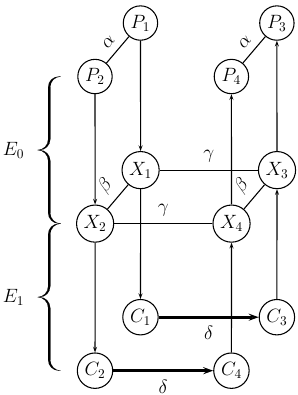
\includegraphics[width=\columnwidth]{images/boomerang.png}
                    \caption{The boomerang attack.}
                    \label{fig:boomerang}
                \end{figure}
            \end{column}
        \end{columns}
    \end{frame}

    \begin{frame}{The Boomerang Distinguisher}
        \vspace{-1em}
        \begin{algorithm}[H]
            \caption{The Boomerang Attack Distinguisher}
            \label{alg:boomerang-dist}
            \begin{algorithmic}[1]
                \State Initialize a counter \(ctr \gets 0\). 
                \State Generate \(\brak{pq}^{-2}\) plaintext pairs \(\brak{P_1, P_2}\)
                such that \(P_1 \oplus P_2 = \alpha\).
                \ForAll {pairs \(\brak{P_1, P_2}\)}
                    \State Ask for the encryption of \(\brak{P_1, P_2}\) to \(\brak{C_1,
                    C_2}\).
                    \State Compute \(C_3 = C_1 \oplus \delta\) and \(C_4 = C_2 \oplus 
                    \delta\). \Comment{\(\delta\)-shift}
                    \State Ask for the decryption of \(\brak{C_3, C_4}\) to \(\brak{P_3,
                    P_4}\).
                    \If {\(P_3 \oplus P_4 = \alpha\)}
                        \State Increment \(ctr\)
                    \EndIf
                \EndFor
                \If {\(ctr > 0\)}
                    \State \Return This is the cipher \(E\)
                \Else
                    \State \Return This is a random permutation
                \EndIf
            \end{algorithmic}
        \end{algorithm}
    \end{frame}

    \subsection{The S-box Switch}
    \label{subsec:s-box-switch}
    
    \begin{frame}[<+->]{Boomerang Switches}
        \begin{enumerate}
            \item Gain 1-2 middle rounds for free by choosing differentials
            carefully. Here, we discuss the \emph{S-box switch}.
            \item Suppose the last operation in \(E_0\) is a layer of S-boxes
            where \(S\brak{\rho_1\|\rho_2\|\ldots\|\rho_t} =
            \brak{f_1\brak{\rho_1}\|f_2\brak{\rho_2}\|\ldots\|f_t\brak{\rho_t}}\)             
            for \(t\) independent keyed functions \(f_i\). Suppose the
            difference for both \(\beta\) and \(\gamma\) corresponding to the
            output of some \(f_j\) is equal to \(\Delta\). 
            \item Denoting this part of the intermediate state by \(X_j\),
            \begin{equation}
                \brak{X_1}_j \oplus \brak{X_2}_j = \brak{X_1}_j \oplus \brak{X_3}_j = \brak{X_2}_j \oplus \brak{X_4}_j = \Delta
                \label{eq:s-switch}
            \end{equation}
            which shows \(\brak{X_1}_j = \brak{X_4}_j\) and \(\brak{X_2}_j =
            \brak{X_3}_j\).
            \item If the differential characteristic in \(f_j^{-1}\) holds for
            \(\brak{X_1, X_2}\), then it will hold for \(\brak{X_3, X_4}\).
            \emph{We pay for probability in one direction}.
            \item Distinguisher probability increases by a factor of
            \(\brak{q^\prime}^{-1}\), where \(q^\prime\) is the probability of
            the differential characteristic in \(f_j\).
        \end{enumerate}
    \end{frame}

    \subsection{The Yoyo Game}
    \label{subsec:yoyo-game}
    
    \begin{frame}[<+->]{The Yoyo Game}
        \begin{enumerate}
            \item Similar to boomerang, starts by encrypting \(\brak{P_1, P_2}\)
            to \(\brak{C_1, C_2}\), then modifying them to \(\brak{C_3, C_4}\)
            and decrypting them.
            \item \emph{Unlike} the boomerang attack, this process continues in
            the yoyo game.
            \item \emph{All} pairs of intermediate values \(\brak{X_{2l + 1},
            X_{2l + 2}}\) satisfy some property (such as zero difference in some
            part).
            \item Probabilities are low with large \(l\). Still, the yoyo
            technique has been used to attack AES reduced to 5 rounds.
        \end{enumerate}
    \end{frame}

    \subsection{Mixture Differentials}
    \label{subsec:mixture}
    
    \begin{frame}{Mixture}
        \begin{definition}[Mixture]
            \label{def:mixture}
            Suppose \(P_i \triangleq \brak{\rho_1^i, \rho_2^i, \ldots,
            \rho_t^i}\). Given a plaintext pair \(\brak{P_1, P_2}\), we say
            \(\brak{P_3, P_4}\) is a \emph{mixture counterpart} of \(\brak{P_1,
            P_2}\) if for each \(1 \le j \le t\), the quartet \(\brak{\rho_j^1,
            \rho_j^2, \rho_j^3, \rho_j^4}\) consists of two pairs of equal
            values or of four equal values. The quartet \(\brak{P_1, P_2, P_3,
            P_4}\) is called a \emph{mixture}.
        \end{definition}
        \pause
        \begin{enumerate}
            \item<2->  If \(\brak{P_1, P_2, P_3, P_4}\) is a mixture, then XOR
            of the intermediate values \(\brak{X_1, X_2, X_3, X_4}\) is zero.
            \item<3-> \(X_1 \oplus X_3 = \gamma \implies X_2 \oplus X_4 =
            \gamma\). Hence, for \(\gamma \xrightarrow{q} \delta\) in \(E_1\),
            \(C_1 \oplus C_3 = C_2 \oplus C_4 = \delta\) with probability
            \(q^2\).
            \item<4-> Has been applied to AES reduced up to 6 rounds. \(E_0\) is
            taken to be the first 1.5 rounds of AES, which can be treated as
            four parallel super S-boxes.
        \end{enumerate}
    \end{frame}

    \section{The Retracing Boomerang Attack}
    \label{sec:retr-boomerang}
    
    \subsection{The Retracing Boomerang Framework}
    \label{sec:retr-framework}

    \begin{frame}{The Retracing Boomerang Framework}
        \begin{figure}[!ht]
            \centering
            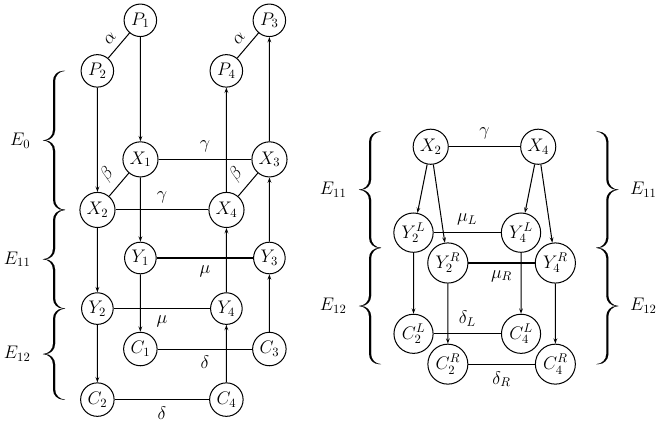
\includegraphics[width=0.6\columnwidth]{images/retracing_boomerang.png}
            \caption{The retracing boomerang attack.}
            \label{fig:retr-boomerang}
        \end{figure}
    \end{frame}

    \begin{frame}[<+->]{The Retracing Boomerang Attack}
        \begin{enumerate}
            \item The \emph{retracing boomerang} framework consists of a
            \emph{shifting} type and a \emph{mixing} type.
            \item Both attacks use the setup shown in \cref{fig:retr-boomerang}.
            \item Although the additional split looks restrictive, it applies
            for a wide class of block ciphers such as SASAS constructions.
            \item Further, we assume that \(E_{12}\) can be split into two parts
            of size \(b\) and \(n - b\) bits, call these functions \(E_{12}^L\)
            and \(E_{12}^R\), with characteristic probabilities \(q_2^L\) and
            \(q_2^R\) respectively.
        \end{enumerate}
    \end{frame}

    \subsection{The Shifting Retracing Attack}
    \label{subsec:shift-retr-boomerang}

    \begin{frame}[<+->]{The Shifting Retracing Boomerang Attack}
        \begin{enumerate}
            \item Adds a \(\brak{b - 1}\)-bit filtering in the middle of the
            attack procedure.
            \item Check if \(C_1^L \oplus C_2^L = 0 \textrm{ or } \delta_L\).
            \emph{Discard all such pairs that do not satisfy this relation}.
            \item A \(\delta\)-shift is performed on the filtered ciphertext
            pairs to get \(\brak{C_3, C_4}\).
            \item Filtering ensures that the two unordered pairs \(\brak{C_1,
            C_3}\) and \(\brak{C_2, C_4}\) are \emph{equal}.
            \item If one of these pairs satisfies the differential
            characteristic \(\delta_L \xrightarrow{q_2^L} \mu_L\), \emph{the
            other pair will too!}.
            \item Increases the probability of the boomerang distinguisher by
            \(\brak{q_2^L}^{-1}\).
            \item Any possible characteristic of \(\brak{E_{12}^L}\) has
            probability at least \(2^{-b + 1}\), thus the overall probability
            increases by a factor of at most \(2^{b - 1}\). On the other hand,
            filtering only leaves \(2^{-b + 1}\) of the pairs, so there is no
            apparent gain.
        \end{enumerate}
    \end{frame}

    \begin{frame}{The Shifting Retracing Boomerang Attack}
        \begin{figure}
            \centering
            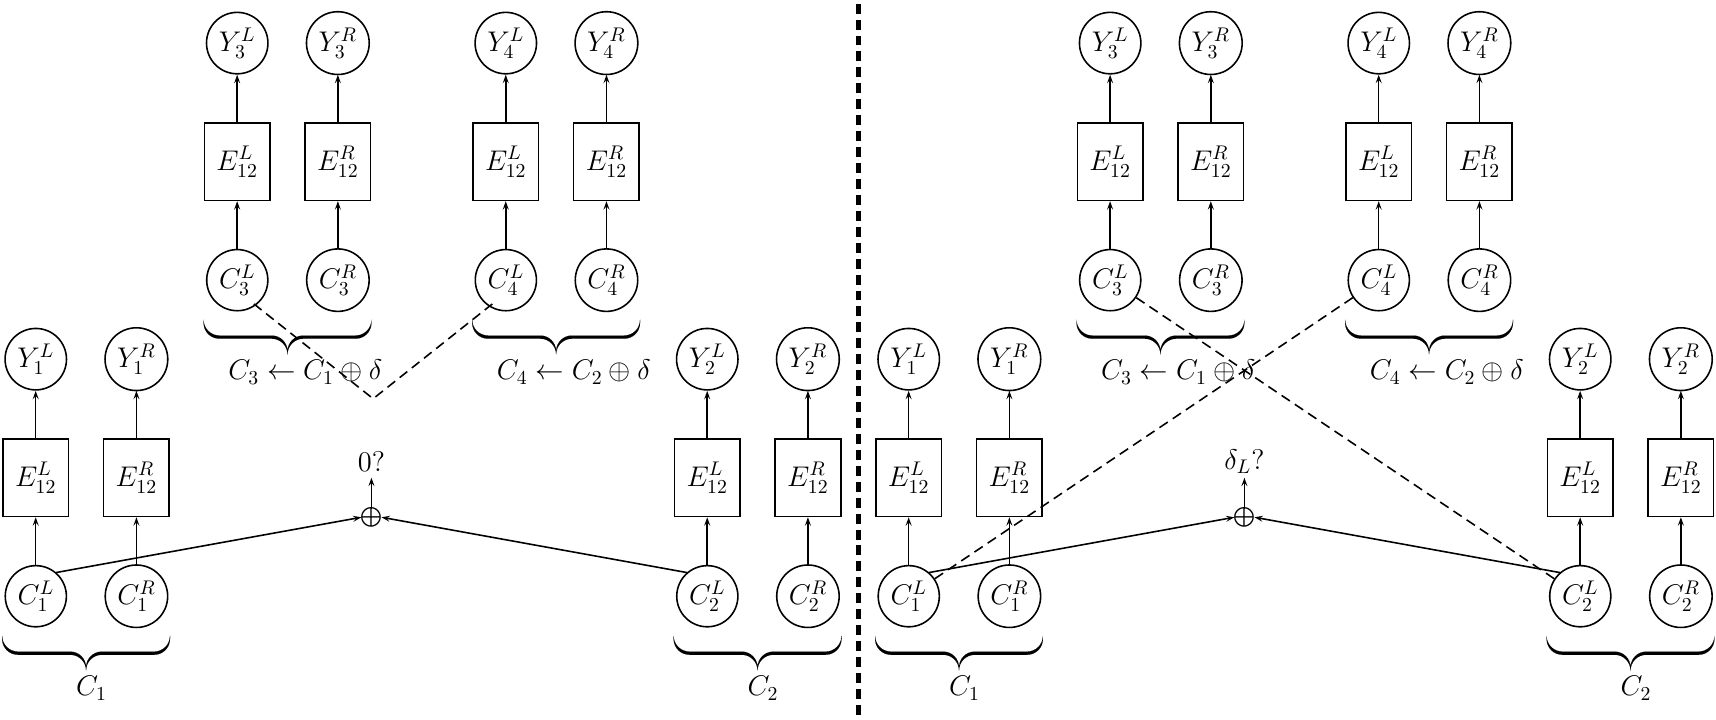
\includegraphics[width=\columnwidth]{images/shifting_boomerang.png}
            \caption{A shifted quartet (dashed lines indicate equality).}
        \end{figure}
    \end{frame}

    \begin{frame}[<+->]{Advantages of Filtering}
        \begin{enumerate}
            \item \emph{Improving the signal to noise ratio.} Improving the
            probability by a factor of \(\brak{q_2^L}^{-1}\) improves the SNR
            which ensures a higher fraction of the filtered pairs on average
            satisfy \(P_3 \oplus P_4 = \alpha\). The characteristic \(\beta
            \xrightarrow{p} \alpha\) in the backward direction for the pair
            \(\brak{X_3, X_4}\) can be replaced by a truncated differential
            characteristic \(\beta \xrightarrow{p^\prime} \alpha^\prime\) of
            higher probability.
            \item \emph{Reducing the data complexity.} Due to the filtering, the
            attack leaves fewer ciphertexts. This improves the complexity in
            cases where more decryption queries are made.
            \item \emph{Reducing the time complexity.} The filtering can also
            reduce the time complexity if it is dominated by the analysis of the
            plaintext pairs \(\brak{P_3, P_4}\).
        \end{enumerate}
    \end{frame}

    \subsection{The Mixing Retracing Attack}
    \label{subsec:mix-retr-boomerang}

    \begin{frame}[<+->]{The Mixing Retracing Boomerang Attack}
        \begin{enumerate}
            \item In the shifting attack, the attacker forces equality between
            the unordered pairs \(\brak{C_1^L, C_2^L}\) and \(\brak{C_3^L,
            C_4^L}\) using a \(\delta\)-shift.
            \item In this type of attack, each ciphertext pair can be shifted by
            \(\brak{C_1^L \oplus C_2^L, 0}\). The resulting ciphertexts are
            \begin{align}
                C_3 &= \brak{C_3^L, C_3^R} = \brak{C_1^L \oplus \brak{C_1^L \oplus C_2^L}, C_1^R} = \brak{C_2^L, C_1^R}, \\
                C_4 &= \brak{C_4^L, C_4^R} = \brak{C_2^L \oplus \brak{C_1^L \oplus C_2^L}, C_2^R} = \brak{C_1^L, C_2^R}.
            \end{align}
            \item Again, the unordered pairs \(\brak{C_1^L, C_2^L}\) and
            \(\brak{C_3^L, C_4^L}\) are equal.
            \item Further, \(C_1^R = C_3^R\) and \(C_2^R = C_4^R\), thus we gain
            an \emph{additional} factor of \(\brak{q_2^R}^{-2}\) for a total
            probability of \(\brak{pq_1}^2q_2^L\), \emph{better than shifting}!
            \item Similar to the core step used in the yoyo attack on AES.
        \end{enumerate}
    \end{frame}

    \begin{frame}{The Mixing Retracing Boomerang Attack}
        \begin{figure}
            \centering
            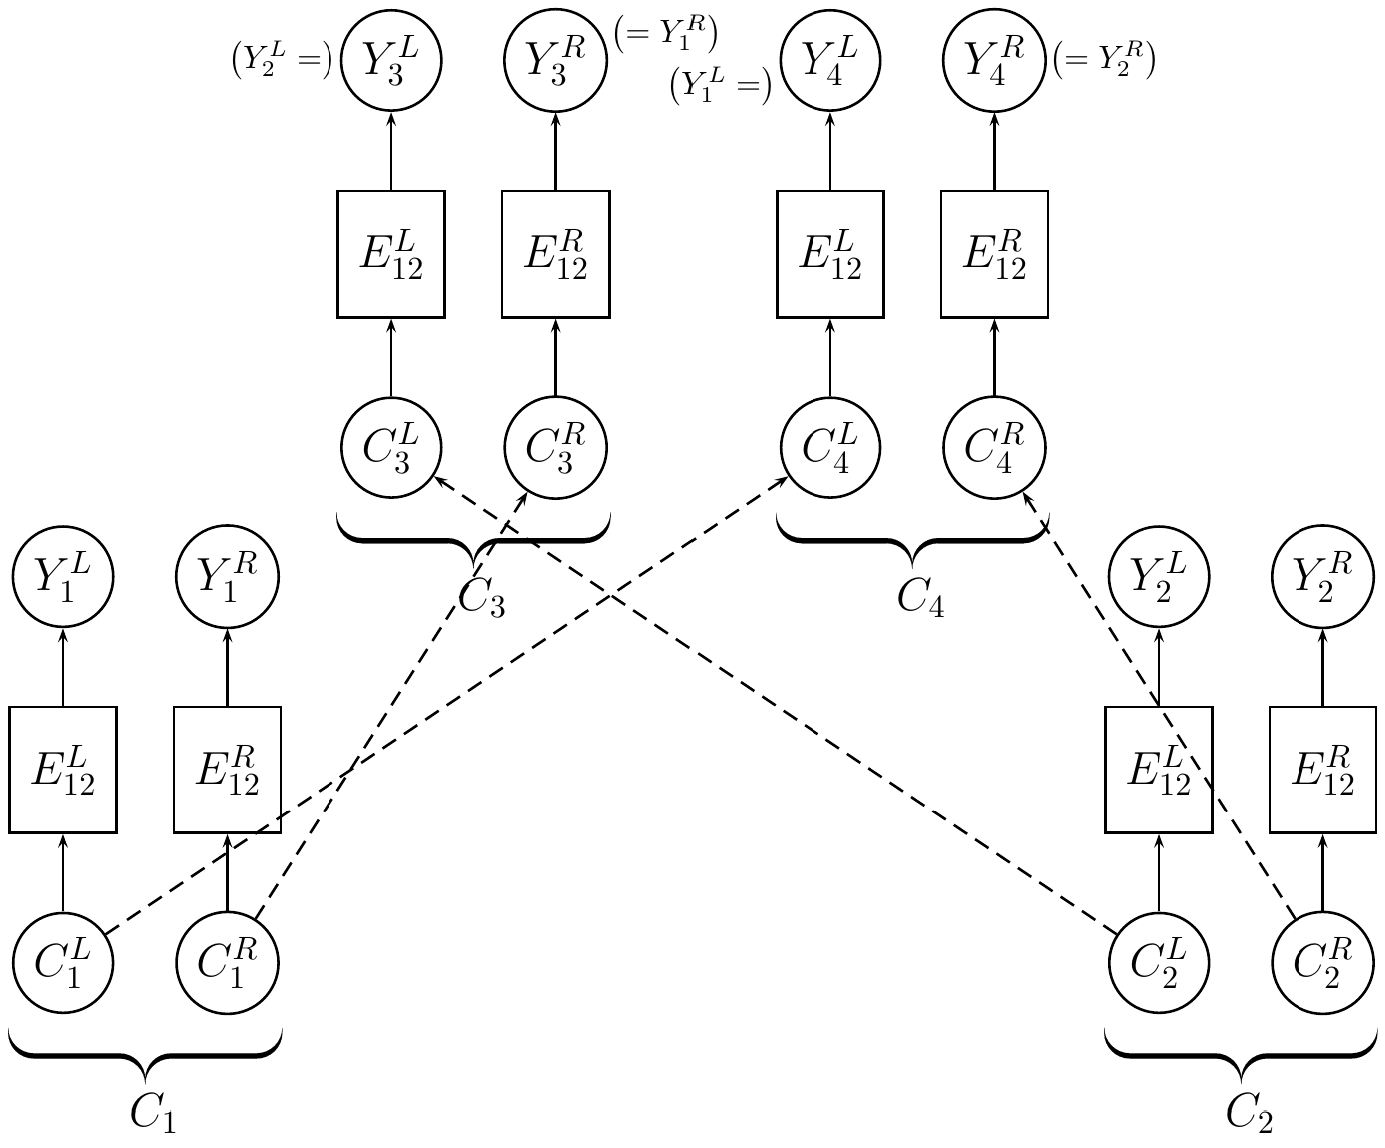
\includegraphics[width=0.55\columnwidth]{images/mixing_boomerang.png}
            \caption{A mixture quartet of ciphertexts (dashed lines indicate equality).}
        \end{figure}
    \end{frame}

    \subsection{Comparison Between the Two Types of Retracing Attacks}
    \label{subsec:cmp}
    \begin{frame}[<+->]{Advantages of Shifting Retracing Attack}
        \begin{enumerate}
            \item \textbf{Using structures}
            \begin{itemize}[<+->]
                \item Shifting applies the same \(\delta\)-shift to all pairs of
                ciphertexts.
                \item Filtering is applied first to reduce the data complexity.
                \item Not possible in mixing: shift is based on ciphertexts, no
                filtering.
                \item Basic boomerang attacks add a round at the top or bottom
                of the distinguisher. With shifting, one can obtain all
                ciphertexts, shift them by \(\delta\) and then decrypt,
                simulatneously checking for the filter and condition between
                \(P_3\) and \(P_4\) using a hash table.
            \end{itemize}
            \item \textbf{Combination with \(E_{11}\)}
            \begin{itemize}[<+->]
                \item In mixing, the output difference of \(E_{12}^L\) is
                arbitrary.
                \item Usually no good combination between characteristics of
                \(\brak{E_{12}^L}^{-1}\) and \(\brak{E_{11}}^{-1}\). For
                instance, in the yoyo attack, \(E_{11}\) is empty.
            \end{itemize}
            \item \textbf{Construction of `friend pairs'}
            \begin{itemize}[<+->]
                \item `Friend pairs' are pairs which satisfy a common property.
                \item More `friend pairs' can be constructed in the shifting
                variant.
            \end{itemize}
        \end{enumerate}
    \end{frame}

    \section[Application to Five Round AES]{Retracing Boomerang Attack on Five Round AES}
    \label{sec:retr-boomerang-aes}

    \subsection{Brief Description of AES}
    \label{subsec:aes-description}

    \begin{frame}{Description of AES}
        \begin{enumerate}[<+->]
            \item Byte ordering shown after \(SB\) in \cref{fig:aes} (column
            major).
            \item \(j\)-th byte of a state \(X_i\) is denoted as \(X_{i,j}\) or
            \(\brak{X_i}_j\).
            \item Denote by \(W, Z\) and \(X\) the states before \(MC\) in round
            0, at the input to round 1 and before \(MC\) in round 2
            respectively.
            \item The \(l\)-th shifted column (resp. \(l\)-th inverse shifted
            column) refers to application of \(SR\) (resp. \(SR^{-1}\)) to the
            \(l\)-th column.
            \item Round subkeys are \(k_{-1}, k_0, \ldots\).
        \end{enumerate}
        \begin{figure}[!ht]
            \centering
            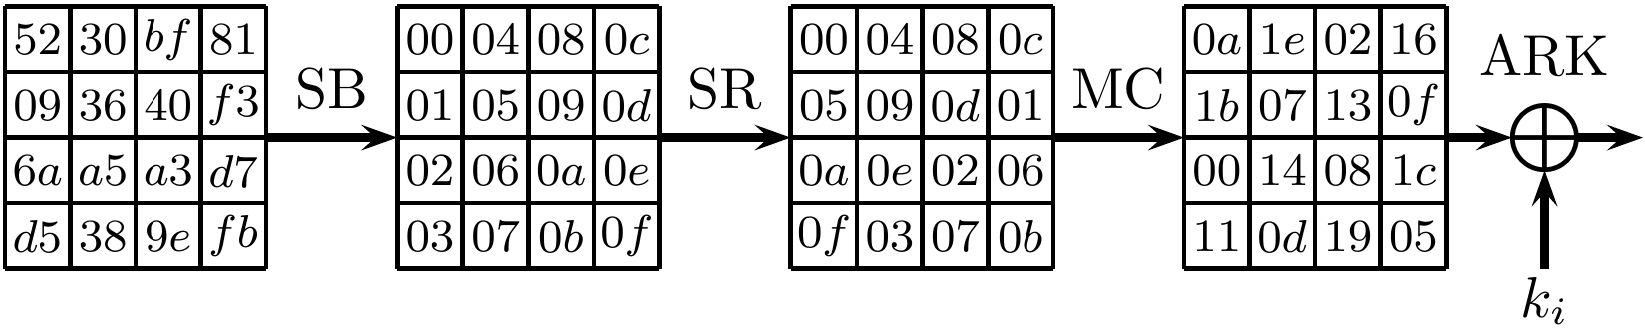
\includegraphics[width=0.85\columnwidth]{images/aes.png}
            \caption{An AES round.}
            \label{fig:aes}
        \end{figure}
    \end{frame}

    \subsection{The Yoyo Attack on Five Round AES}
    \label{subsec:yoyo-aes}

    \begin{frame}[<+->]{Summary of Yoyo Attack on Five Round AES}
        \begin{enumerate}
            \item Decomposes AES as \(E = E_{12} \circ E_{11} \circ E_0\) where
            \(E_0\) is the first 2.5 rounds, \(E_{11}\) is the MC of round 2 and
            \(E_{12}\) is the last 2 rounds.
            \item Truncated differential characteristic for \(E_0\): zero input
            difference in three inverse shifted columns and zero output
            difference in a single shifted column with probability \(4 \cdot
            2^{-8} = 2^{-6}\). (\emph{why?})
            \item For \(E_{12}\), 1.5 rounds of AES can be taken as four 32-bit
            super S-boxes.
            \item Ciphertext pair \(\brak{C_1, C_2}\) modified into its mixture
            \(\brak{C_3, C_4}\) w.r.t. super S-boxes and decrypted. The four
            inputs to the S-boxes have zero XOR, thus \(X_1 \oplus X_2 \oplus
            X_3 \oplus X_4 = 0\) since MC is linear. 
            \item \(X_3 \oplus X_4 = 0\) in a shifted column and \(Z_3 \oplus
            Z_4 = 0\) in an inverse shifted column with probability \(2^{-6}\).
            This corresponds to one of the four quartets \(\brak{0,5,10,15}\),
            \(\brak{1,4,11,14}\), \(\brak{2,5,8,13}\), \(\brak{3,6,9,12}\).
            \item Attack quartets of \(k_{-1}\). Friend pairs of \(\brak{Z_3,
            Z_4}\) used to get more information.
        \end{enumerate}
    \end{frame}

    \begin{frame}{Algortihm of Yoyo Attack}
        \begin{algorithm}[H]
            \caption{Yoyo Attack on Five Round AES}
            \label{alg:yoyo-aes}
            \algrenewcommand\alglinenumber[1]{\scriptsize ####1:}
            \scriptsize
            \begin{algorithmic}[1]
                \State Ask for the encryption of \(2^6\) pairs \(\brak{P_1,
                P_2}\) of chosen plaintexts with non-zero difference only in 
                bytes \(0, 5, 10, 15\).
                \For {all corresponding ciphertext pairs \(\brak{C_1, C_2}\)}
                    \State Let \(\brak{C_3^j, C_4^j}\), \(j = 1, 2, 3, 4\) be
                    the mixture counterparts of the pair \(\brak{C_1, C_2}\).
                    \State Ask for the decryption of the ciphertext pairs and
                    consider the pairs \(\brak{Z_3^j, Z_4^j}\).
                    \ForAll {\(l \in \cbrak{0, 1, 2, 3}\)}
                        \State Assume all four pairs \(\brak{Z_3^j, Z_4^j}\) and
                        the pair \(\brak{Z_1, Z_2}\) have zero difference in 
                        byte \(l\).
                        \State Use the assumption to extract bytes \(0, 5, 10,
                        15\) of \(k_{-1}\).
                        \If {a contradiction is reached}
                            \State Increment \(l\)
                            \If {\(l > 3\)}
                                Discard the pair
                            \EndIf
                        \Else
                            \State Using \(Z_3^j \oplus Z_4^j = 0\) in the
                            entire \(l\)-th inverse shifted column, attack the
                            three remaining columns of round 0 (sequentially)
                            and decude the rest of \(k_{-1}\).
                        \EndIf
                    \EndFor
                \EndFor
            \end{algorithmic}
        \end{algorithm}
    \end{frame}

    \begin{frame}[<+->]{Meet in the Middle Improvement on Yoyo Attack}
        \begin{enumerate}
            \item Data complexity of \(2^9\) and time complexity of \(2^{40}\).
            Careful analysis of round 0 can reduce the complexity down to
            \(2^{31}\).
            \item Can improve using a meet in the middle (MITM) attack on bytes
            0, 5, 10 and 15 of \(k_{-1}\).
            \item Denote the value of byte \(m\) before \(MC\) operation of
            round 0 by \(W_m\), and WLOG let \(l = 0\). Then,
            \begin{equation}
                Z_0 = 02_x \cdot W_0 \oplus 03_x \cdot W_1 \oplus 01_x \cdot W_2 \oplus 01_x \cdot W_3.
                \label{eq:mitm}
            \end{equation}
            \item The adversary guesses bytes 0, 5 of \(k_{-1}\) by computing
            the following for \(j = 1, 2, 3\) and storing the concatenated
            24-bit value in a hash table.
            \begin{equation}
                02_x \cdot \brak{\brak{W_3^j}_0 \oplus \brak{W_4^j}_0} \oplus 03_x \cdot \brak{\brak{W_3^j}_1 \oplus \brak{W_4^j}_1}
                \label{eq:mitm-0-5}
            \end{equation}
            \seti
        \end{enumerate} 
    \end{frame}

    \begin{frame}[<+->]{Meet in the Middle Improvement on Yoyo Attack}
        \begin{enumerate}
            \conti
            \item Similarly, the adversary does this for bytes 10, 15 of
            \(k_{-1}\), computing
            \begin{equation}
                01_x \cdot \brak{\brak{W_3^j}_2 \oplus \brak{W_4^j}_2} \oplus 01_x \cdot \brak{\brak{W_3^j}_3 \oplus \brak{W_4^j}_3}
                \label{eq:mitm-10-15}
            \end{equation}
            \item The adversary checks for a match in the table, which is
            equivalent to \(\brak{Z_3^j}_0 = \brak{Z_4^j}_0\) for \(j = 1, 2,
            3\).
            \item 24-bit filtering leaves \(2^8\) candidates for bytes 0, 5, 10,
            15 of \(k_{-1}\), checked using the conditions \(\brak{Z_3^4}_0 =
            \brak{Z_4^4}_0\) and \(\brak{Z_1}_0 = \brak{Z_2}_0\).
            \item Although the data complexity looks like \(2^{16}\), the
            \emph{dissection technique} can be used to maintain the memory at
            \(2^9\).
            \item The time complexity is now reduced to \(2^6 \cdot 4 \cdot
            2^{16} = 2^{24}\) operations, which is roughly equivalent to less
            than \(2^{23}\) encryptions.
        \end{enumerate} 
    \end{frame}

    \subsection{Improved Attack on Five Round AES}
    \label{subsec:improved-mitm}

    \begin{frame}[<+->]{Improving the MITM Attack}
        \begin{enumerate}
            \item The MITM attack can be improved to a time complexity of
            \(2^{16.5}\) at the expense of incereasing the data complexity to
            \(2^{15}\).
            \item The main idea is to reduce the number of possible key values
            to \(2^8\) instead of \(2^{16}\) as described earlier. This is done
            in multiple steps.
            \begin{itemize}
                \item Specific choice of plaintexts based on DDT of AES S-boxes.
                \item Eliminating key bytes using friend pairs.
            \end{itemize}
        \end{enumerate}
    \end{frame}

    \begin{frame}[<+->]{Specific Choice of Plaintexts}
        \begin{enumerate}
            \item Choose plaintexts with non-zero difference \emph{only in bytes
            0 and 5.} Here, \(\brak{Z_1}_0 = \brak{Z_2}_0\) leaves \(2^8\)
            candidates for \(k_{-1, \cbrak{0, 5}}\), given by
            \begin{equation}
                02_x \cdot \brak{\brak{W_1}_0 \oplus \brak{W_2}_0} \oplus 03_x \cdot \brak{\brak{W_1}_1 \oplus \brak{W_2}_1} = 0.
                \label{eq:mitm-simple}
            \end{equation}
            \item Constrain \(\brak{P_1}_5 \oplus \brak{P_2}_5 = 01_x\) to
            detect right key bytes efficiently.
            \item DDT row of AES S-box for input difference \(01_x\) along with
            input pair(s) for each output difference computed and stored in
            memory.
            \item For each \(\brak{P_1, P_2}\) and for each guess of \(k_{-1,
            0}\), use \eqref{eq:mitm-simple} to compute the output difference of
            the SB operation in byte 5.
            \item We can lookup to find inputs that can lead to this difference
            and retrieve possible values of \(k_{-1, 5}\) that correspond to the
            guessed \(k_{-1, 0}\).
            \item Gives \(2^8\) values of \(k_{-1, \cbrak{0, 5}}\) in about
            \(2^8\) simple operations per pair.
        \end{enumerate}        
    \end{frame}

    \begin{frame}[<+->]{Eliminating Key Bytes Using Friend Pairs}
        \begin{enumerate}
            \item To reduce the number of candidates for \(k_{-1, \cbrak{10,
            15}}\), the boomerang process is used to return multiple friend
            pairs \(\brak{P_3^j, P_4^j}\).
            \item In particular, we choose one such pair for which
            \begin{equation}
                \brak{P_3^j}_{10} \oplus \brak{P_4^j}_{10} = 0 \quad \textrm{or} \quad \brak{P_3^j}_{15} \oplus \brak{P_4^j}_{15} = 0.
                \label{eq:mitm-check}
            \end{equation}
            Assume WLOG that equality holds in byte 10.
            \item Then, \eqref{eq:mitm-10-15} depends only on \(k_{-1, 15}\) and
            has only \(2^8\) possible values.
            \item Requires \(2^9\) simple operations and leaves \(2^8\)
            candidates for \(k_{-1, \cbrak{0, 5, 15}}\).
            \item Similar MITM procedure followed with another friend pair to
            obtain the unique value of \(k_{-1, \cbrak{0, 5, 10, 15}}\) by
            isolating \(k_{-1, 10}\).
            \item Perform \(2^8\) operations for each pair \(\brak{P_1, P_2}\)
            and for each value of \(l\). Total time complexity of about
            \(2^{16}\) operations.
            \item Each pair requires \(2^7\) friend pairs to find one that
            satisfies \eqref{eq:mitm-check} with high probability. Total data
            complexity is increased to about \(2^{15}\).
        \end{enumerate} 
    \end{frame}

    \begin{frame}[<+->]{Attack Algorithm}
        \begin{enumerate}
            \item \textbf{Precomputation:} Compute DDT row of AES S-box for
            input difference \(01_x\), along with actual inputs for each output
            difference.
            \item \textbf{Online Phase:} Take 64 pairs \(\brak{P_1, P_2}\) with
            \(\brak{P_1}_5 = 00_x\), \(\brak{P_2}_5 = 01_x\), \(\brak{P_1}_0 \ne
            \brak{P_2}_0\) and all other corresponding bytes equal.
            \item For each plaintext pair, create \(2^7\) friend pairs
            \(\brak{P_1^j, P_2^j}\) such that for each \(j\), \(P_1^j \oplus
            P_2^j = P_1 \oplus P_2\) and \(\brak{P_1^j}_{\cbrak{0, 5, 10, 15}} =
            \brak{P_1}_{\cbrak{0, 5, 10, 15}}\).
            \seti
        \end{enumerate}
    \end{frame}

    \begin{frame}[<+->]{Attack Algorithm}
        \begin{enumerate}
            \conti
            \item For each plaintext pair \(\brak{P_1, P_2}\) and for each \(l
            \in \cbrak{0, 1, 2, 3}\), do the following. (\(l = 0\) taken below)
            \begin{enumerate}[<+->]
                \item Use \eqref{eq:mitm-simple} to compute and store all
                \(2^8\) candidates for \(k_{-1, \cbrak{0, 5}}\) in a table.
                \item Use the boomerang process to obtain pairs \(\brak{P_3,
                P_4}\) and \(\brak{P_3^j, P_4^j}\).
                \item Find a \(j\) for which \eqref{eq:mitm-check} is satisfied.
                Perform an MITM attack on column 0 of round 0 using
                \(\brak{P_3^j, P_4^j}\) to obtain \(2^8\) candidates for
                \(k_{-1, \cbrak{0, 5, 15}}\).
                \item Perform another MITM attack on column 0 of round 0 using
                two plaintext pairs \(\brak{P_3^{j^\prime}, P_4^{j^\prime}}\).
                This gives a possible value for \(k_{-1, \cbrak{0, 5, 10,
                15}}\).
                \item If contradiction, go to the next value of \(l\). If
                contradiction for all \(l\), discard this pair and go to the
                next pair.
            \end{enumerate}
            \item Using a pair \(\brak{P_1, P_2}\) for which no contradiction
            occurred, perform similar MITM attacks on columns 1, 2 and 3 of
            round 0 using the fact that \(Z_3 \oplus Z_4\) equals 0 in the
            \(l\)-th inverse shifted column to recover the entire \(k_{-1}\). 
        \end{enumerate}
    \end{frame}

    \begin{frame}[<+->]{Attack Analysis}
        \begin{enumerate}
            \item The attack succeeds if the data contains a pair that satisfies
            the truncated differential characteristic of \(E_0\) and for one of
            the `friend pairs' of that pair, the corresponding plaintext pair
            \(\brak{P_3^j, P_4^j}\) has zero difference in either byte 10 or 15.
            \item Increasing the number of initial pairs and friend pairs per
            initial pair boosts success probability. With 64 pairs and 128
            friend pairs per initial pair, the probability of success is
            \(\brak{1 - e^{-1}}^2 \approx 0.4\)
            \item Another way to boost succees probability is to find other ways
            to cancel terms in \eqref{eq:mitm-10-15}. For instance, if there
            exist \(j, j^\prime\) such that \(\cbrak{\brak{P_3^j}_{10},
            \brak{P_4^j}_{10}} = \cbrak{\brak{P_3^{j^\prime}}_{10},
            \brak{P_4^{j^\prime}}_{10}}\), we can take the XOR of
            \eqref{eq:mitm-10-15} to cancel the effect of \(k_{-1, 10}\), thus
            increasing the success probability even when there is no pair that
            satisfies \eqref{eq:mitm-check}.
            \seti
        \end{enumerate} 
    \end{frame}

    \begin{frame}[<+->]{Attack Analysis}
        \begin{enumerate}
            \conti
            \item Data complexity is \(2 \cdot 2^6 \cdot 2^7 = 2^{14}\) chosen
            plaintexts and \(2^{14}\) adaptively chosen ciphertexts.
            \item Structures can reduce the data complexity to slightly above
            \(2^{14}\) adaptively chosen ciphertexts and plaintexts, but also
            slightly reduces the success probability due to additional
            dependencies between analyzed pairs.
            \item Memory complexity of the attack remains at \(2^9\) 128-bit
            memory cells, like the yoyo attack.
            \item Time complexity is dominated by several MITM attacks that take
            \(2^{16}\) operations each. Considering one AES operation to be
            equivalent to 80 S-box lookups and adding it to the number of
            queries gives us a total of \(2^{16.5}\) encryptions.
        \end{enumerate} 
    \end{frame}

    \section[Secret S-Boxes]{Improved Attack on Five Round AES with a Secret S-box}
    \label{sec:secret-s-box}

    \begin{frame}[<+->]{Attack on Five Round AES with a Secret S-box}
        \begin{enumerate}
            \item Retracing boomerang attack recovers the secret key without
            fully recovering the secret S-box (the S-box is recovered upto an
            affine transformation in \(GF\brak{2^8}\)).
            \item The idea exploit the fact that with probability \(2^{-6}\),
            the pair \(\brak{Z_3, Z_4}\) has zero difference in an inverse
            shifted column.
            \item This observation does not depend on the specific structure of
            \(MC\) and \(SB\) operations, hence it can be applied to
            key-dependent variants as well.
        \end{enumerate}
    \end{frame}

    \begin{frame}[<+->]{Setting up a System of Linear Equations}
        \begin{enumerate}
            \item Assume WLOG the retracing boomerang produces zero difference
            in byte 0 of state \(Z\), or \(\brak{Z_3}_0 \oplus \brak{Z_4}_0 =
            0\). \eqref{eq:mitm} can be rewritten as
            \begin{align}
                0 ={}&\brak{Z_3}_0 \oplus \brak{Z_4}_0 \\
                \begin{split}
                    ={}& 02_x \cdot \brak{\brak{W_3}_0 \oplus \brak{W_4}_0} \oplus 03_x \cdot \brak{\brak{W_3}_1 \oplus \brak{W_4}_1} \\
                    &\oplus 01_x \cdot \brak{\brak{W_3}_2 \oplus \brak{W_4}_2} \oplus 01_x \cdot \brak{\brak{W_3}_3 \oplus \brak{W_4}_3}.
                \end{split}
                \label{eq:lin-secret}
            \end{align}
            \item Note that \(\brak{W_3}_j = SB\brak{P_3 \oplus k_{-1,
            j^\prime}}\) for \(j = 0, 1, 2, 3\) where \(j^\prime =
            SR^{-1}\brak{j}\).
            \item If we define \(4 \cdot 256 = 1024\) variables \(x_{m,j} =
            SB\brak{m \oplus k_{-1, j^\prime}}\) for \(m \in \bF_q\) and \(j =
            0, 1, 2, 3\), then each plaintext pair \(P_1, P_2\) which satisfies
            \eqref{eq:lin-secret} provides a linear equation in the variables
            \(x_{m,j}\).
            \seti
        \end{enumerate}    
    \end{frame}

    \begin{frame}[<+->]{Setting up a System of Linear Equations}
        \begin{enumerate}
            \conti
            \item To obtain many pairs, attach about \(2^{10}\) friend pairs to
            each of the \(2^6\) original pairs \(\brak{P_1, P_2}\).
            \item For each original pair along with its friend pairs, perform
            the mixing retracing boomerang process to obtain a linear equation
            in the variables \(x_{m, j}\). A few more friend pairs are taken for
            extra filtering of the original pairs.
            \item Since differences are used \eqref{eq:lin-secret}, we can
            recover the S-box with an invertible linear transformation over
            \(GF\brak{2^8}\). That is, we can only obtain functions \(S_0, S_1,
            S_2, S_3\) such that
            \begin{equation}
                S_j\brak{x} = L_0\brak{SB\brak{x \oplus k_{-1, j^\prime}}},
            \end{equation}
            for some unknown linear transformation \(L_0\). Similar linear
            transformations \(L_t\) will be obtained for column \(t\).
        \end{enumerate}    
    \end{frame}

    \begin{frame}[<+->]{Recovering the Secret Key}
        \begin{enumerate}
            \item First, for each \(j^\prime\), we can recover 
            \(\bar{k_{j^\prime}} = k_{-1, 0} \oplus k_{-1, {j^\prime}}\) as 
            \(\bar{k_{j^\prime}}\) is the unique value of \(c\) such that
            \(S_j\brak{x} = S_0\brak{x \oplus c}\) for all \(x\).
            \item Similarly, we can recover each inverse shifted column of
            \(k_{-1}\) up to \(2^8\) possible values, reducing the total number
            of candidates to \(2^{32}\).
            \item Second, the differences \(k_{-1, 0} \oplus k_{-1, j}\) for
            \(j = 1, 2, 3\) can be found by taking quartets \(\brak{x_0, x_1,
            x_2, x_3}\) such that \(\bigoplus_{i=0}^3S_0\brak{x_i} = 0\).
            \item Quartets eliminate the effect of the difference between the
            linear transformations \(L_0\) and \(L_j\) by finding the unique
            \(c_j\) such that \(\bigoplus_{i=0}^3 S_j\brak{c_j \oplus x} = 0\).
            \item Thus, in about \(2^{12}\) operations, we can determine the 
            entire secret key \(k_{-1}\) upto the value of \(k_{-1, 0}\), 
            giving \(2^8\) possibilities to be exhaustively searched.
        \end{enumerate}
    \end{frame}

    \begin{frame}[<+->]{Attack Analysis}
        \begin{enumerate}
            \item Data complexity is \(2 \cdot 2^6 \cdot 2^{10} = 2^{17}\)
            chosen plaintexts and \(2^{17}\) adaptively chosen ciphertexts.
            \item Using structures, the amount of chosen plaintexts can be
            reduced to \(2^{14}\), thus the overall data complexity is less
            than \(2^{17.5}\) chosen plaintexts and adaptively chosen
            ciphertexts.
            \item The time complexity is dominated by solving a system
            of 1034 equations in 1024 variables for each of the \(2^6\) pairs
            \(\brak{P_1, P_2}\). Using an efficient algorithm such as the
            Method of the Four Russians, each solution takes about \(2^{27}\)
            simple operations or approximately \(2^{21}\) encryptions. Thus,
            the overall time complexity is \(2^{29}\).
            \item The memory complexity is dominated by the memory required for
            solving the equations, which is about \(2^{17}\) 128-bit blocks.
        \end{enumerate}
    \end{frame}

    \begin{frame}[<+->]{Improvement From Distinguisher}
        \begin{enumerate}
            \item The equation solving step has to be applied \(2^8\) times
            since we do not know if a pair satisfies the boomerang property.
            \item To obtain this information in advance, we can use the 
            five-round yoyo distinguisher.
            \item In this variant, the time complexity is dominated by the 
            complexity of the yoyo distinguisher, which is \(2^{25.8}\). The
            memory complexity is still \(2^{17}\).
        \end{enumerate}
    \end{frame}

    \section[Retracing Rectangle Attack]{The Retracing Rectange Attack and Mixture Differentials}
    \label{sec:retracing-rectangle}
    
    \subsection{The Amplified Boomerang Attack}
    \label{subsec:amplified-boomerang}

    \begin{frame}[<+->]{Amplified Boomerang Attack}
        \begin{enumerate}
            \item Retracing boomerang attack uses the stronger adaptively
            chosen plaintext and ciphertext model.
            \item Amplified boomerang attack uses only the chosen plaintext
            model of attack.
            \item In this version of the boomerang attack, the adversary 
            considers \emph{pairs of pairs} of plaintexts 
            \(\brak{\brak{P_1, P_2}, \brak{P_3, P_4}}\) such that \(P_1 \oplus
            P_2 = P_3 \oplus P_4 = \alpha\). For each pair, the adversary
            checks whether the corresponding quartet of ciphertexts
            \(\brak{\brak{C_1, C_2}, \brak{C_3, C_4}}\) satisfy \(C_1 \oplus
            C_2 = C_3 \oplus C_4 = \delta\).
            The analysis behind this distinguisher is that the overall probability of the
            boomerang is \(p^2q^2\), thus if \(pq \gg 2^{-n/2}\), then a distinguisher can
            be created using \(4 \cdot 2^{n/2}\brak{pq}^{-1}\) chosen plaintexts. The time
            complexity of this attack is \(\cO\brak{2^{n/2}\brak{pq}^{-1}}\) using hash
            tables.

        \end{enumerate}
    \end{frame}
\subsection{The Retracing Rectangle Attack}

Translating a retracing boomerang attack to a retracing rectangle attack follows
the same idea as translating a (classical) boomerang attack to a rectangle
attack. We start with decomposing \(E = E_1 \circ E_{02} \circ E_{01}\), where
\(E_{01}\) divides the state into two parts of \(b\) and \(n - b\) bits.
Further, suppose that there exists differential characteristics \(\alpha_L
\xrightarrow{p_1^L} \mu_L\) for \(E_{01}^L\), \(\alpha_R \xrightarrow{p_1^R}
\mu_R\) for \(E_{01}^R\), \(\mu \xrightarrow{p_2} \beta\) for \(E_{02}\) and
\(\gamma \xrightarrow{q} \delta\) for \(E_1\). This is illustrated in
\autoref{fig:retr-rectangle}.

\begin{figure}
    \centering
    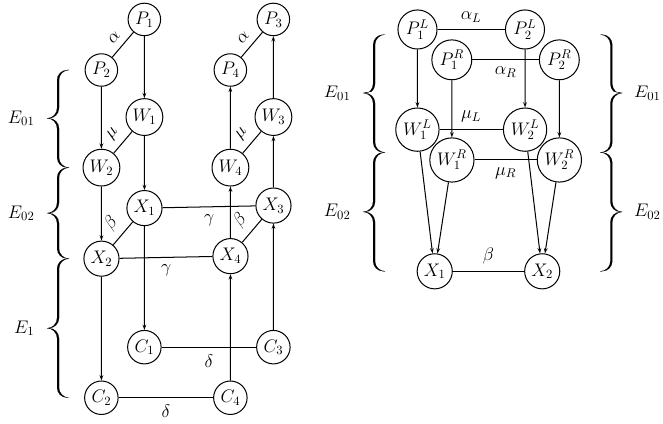
\includegraphics[width=0.6\columnwidth]{images/retracing_rectangle.png}
    \caption{The retracing rectangle attack.}
    \label{fig:retr-rectangle}
\end{figure}

A distinguisher can be built assuming \(p_1^Lp_1^Rp_2q \gg 2^{-n/2}\) as before.
However, in the retracing rectangle attack, we consider plaintext quartets that
satisfy
\begin{equation}
    \brak{P_1 \oplus P_2 = \alpha} \land \brak{P_3 \oplus P_4 = \alpha} \land \brak{P_1^L \oplus P_3^L = 0 \textrm{ or } \alpha_L}.
    \label{eq:retr-rect-cond}
\end{equation}
As a result of \eqref{eq:retr-rect-cond}, \(\cbrak{P_1^L, P_2^L} = \cbrak{P_3^L,
P_4^L}\). If one of them satisfies the differential characteristic of
\(E_{10}^L\), then so does the other. This improves the probability of the
distinguisher by a factor of \(\brak{p_1^L}^{-1}\).

Unlike the shifting retracing boomerang attack, there is no need to filter data
to obtain an improvement. Additionally, the signal to noise ratio is improved.
Usually, the adversary starts with a structure \(\cS\) of plaintext pairs with
input difference \(\alpha\). Instead of checking all \(\binom{\abs{\cS}}{2}\)
pairs, a hash table is used to check all quartets in \(\cO\brak{\abs{\cS}}\)
time.

\subsection{Mixing Variant and Relation to Mixture Differentials}

Similar to the mixing retracing boomerang attack, the adversary can force,
\(\cbrak{P_1^L, P_2^L} = \cbrak{P_3^L, P_4^L}\) by choosing \(P_3 = \brak{P_2^L,
P_1^R}\) and \(P_4 = \brak{P_1^L, P_2^R}\). As this choice forces
\(\cbrak{P_1^R, P_2^R} = \cbrak{P_3^R, P_4^R}\), the probability of the
rectangle distinguisher is increased by a factor of \(\brak{p_1^Lp_1^R}^{-1}\).

    \section{The Retracing Rectange Attack and Mixture Differentials}

A drawback of the retracing boomerang attack is that it uses the stronger
adaptively chosen plaintext and ciphertext model. However, the amplified
boomerang attack uses only the chosen plaintext model of attack. We first
explore this attack before introducing the retracing variant.

\subsection{The Amplified Boomerang Attack}

In this version of the boomerang attack, the adversary considers \emph{pairs of
pairs} of plaintexts \(\brak{\brak{P_1, P_2}, \brak{P_3, P_4}}\) such that \(P_1
\oplus P_2 = P_3 \oplus P_4 = \alpha\). For each such pair, the adversary then
checks whether the corresponding quartet of ciphertexts \(\brak{\brak{C_1, C_2},
\brak{C_3, C_4}}\) satisfy \(C_1 \oplus C_2 = C_3 \oplus C_4 = \delta\).

The analysis behind this distinguisher is that the overall probability of the
boomerang is \(p^2q^2\), thus if \(pq \gg 2^{-n/2}\), then a distinguisher can
be created using \(4 \cdot 2^{n/2}\brak{pq}^{-1}\) chosen plaintexts. The time
complexity of this attack is \(\cO\brak{2^{n/2}\brak{pq}^{-1}}\) using hash
tables.

\subsection{The Retracing Rectangle Attack}

Translating a retracing boomerang attack to a retracing rectangle attack follows
the same idea as translating a (classical) boomerang attack to a rectangle
attack. We start with decomposing \(E = E_1 \circ E_{02} \circ E_{01}\), where
\(E_{01}\) divides the state into two parts of \(b\) and \(n - b\) bits.
Further, suppose that there exists differential characteristics \(\alpha_L
\xrightarrow{p_1^L} \mu_L\) for \(E_{01}^L\), \(\alpha_R \xrightarrow{p_1^R}
\mu_R\) for \(E_{01}^R\), \(\mu \xrightarrow{p_2} \beta\) for \(E_{02}\) and
\(\gamma \xrightarrow{q} \delta\) for \(E_1\). This is illustrated in
\autoref{fig:retr-rectangle}.

\begin{figure}
    \centering
    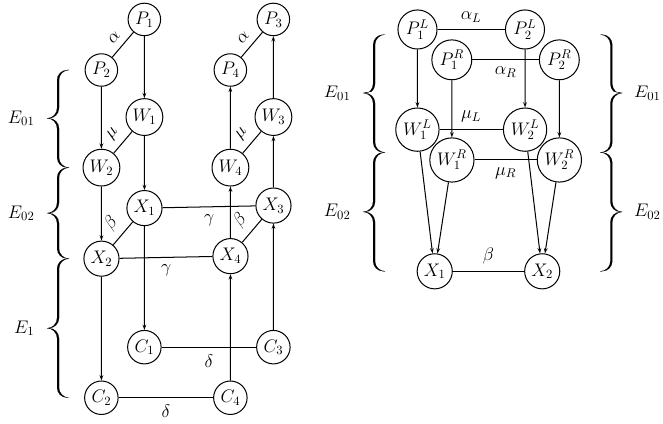
\includegraphics[width=0.6\columnwidth]{images/retracing_rectangle.png}
    \caption{The retracing rectangle attack.}
    \label{fig:retr-rectangle}
\end{figure}

A distinguisher can be built assuming \(p_1^Lp_1^Rp_2q \gg 2^{-n/2}\) as before.
However, in the retracing rectangle attack, we consider plaintext quartets that
satisfy
\begin{equation}
    \brak{P_1 \oplus P_2 = \alpha} \land \brak{P_3 \oplus P_4 = \alpha} \land \brak{P_1^L \oplus P_3^L = 0 \textrm{ or } \alpha_L}.
    \label{eq:retr-rect-cond}
\end{equation}
As a result of \eqref{eq:retr-rect-cond}, \(\cbrak{P_1^L, P_2^L} = \cbrak{P_3^L,
P_4^L}\). If one of them satisfies the differential characteristic of
\(E_{10}^L\), then so does the other. This improves the probability of the
distinguisher by a factor of \(\brak{p_1^L}^{-1}\).

Unlike the shifting retracing boomerang attack, there is no need to filter data
to obtain an improvement. Additionally, the signal to noise ratio is improved.
Usually, the adversary starts with a structure \(\cS\) of plaintext pairs with
input difference \(\alpha\). Instead of checking all \(\binom{\abs{\cS}}{2}\)
pairs, a hash table is used to check all quartets in \(\cO\brak{\abs{\cS}}\)
time.

\subsection{Mixing Variant and Relation to Mixture Differentials}

Similar to the mixing retracing boomerang attack, the adversary can force,
\(\cbrak{P_1^L, P_2^L} = \cbrak{P_3^L, P_4^L}\) by choosing \(P_3 = \brak{P_2^L,
P_1^R}\) and \(P_4 = \brak{P_1^L, P_2^R}\). As this choice forces
\(\cbrak{P_1^R, P_2^R} = \cbrak{P_3^R, P_4^R}\), the probability of the
rectangle distinguisher is increased by a factor of \(\brak{p_1^Lp_1^R}^{-1}\).

\end{document}
